% Chapter 4. OAuth 2.1 as MCP uses it, with the round trips counted.
\documentclass[tikz,border=6pt]{standalone}
% Shared look for every TikZ figure in the book.
% Colours match book/preamble.tex exactly. Change both or neither.

\usepackage{tikz}
\usepackage{xcolor}
\usepackage{amsmath}
\IfFileExists{libertinus.sty}{\usepackage[mono=false]{libertinus}}{}
\IfFileExists{inconsolata.sty}{\usepackage[varqu,varl,scaled=0.95]{inconsolata}}{}

\usetikzlibrary{
  arrows.meta, positioning, calc, fit, backgrounds, shapes.geometric,
  shapes.misc, decorations.pathreplacing, decorations.pathmorphing,
  patterns, chains, matrix, shadows.blur
}

\definecolor{ink}{HTML}{15181D}
\definecolor{muted}{HTML}{5B6472}
\definecolor{rule}{HTML}{C9CED6}
\definecolor{wash}{HTML}{F4F5F7}
\definecolor{accent}{HTML}{0F5C8C}
\definecolor{accentsoft}{HTML}{E7F0F6}
\definecolor{warm}{HTML}{B4531A}
\definecolor{warmsoft}{HTML}{FBF0E7}
\definecolor{good}{HTML}{2C6E49}
\definecolor{goodsoft}{HTML}{E9F2EC}
\definecolor{danger}{HTML}{9B2226}
\definecolor{dangersoft}{HTML}{FAECEC}

\tikzset{
  font=\sffamily\small,
  >={Stealth[length=5pt, width=4pt]},
  %
  box/.style={
    draw=rule, line width=0.8pt, fill=wash, rounded corners=2pt,
    inner sep=7pt, align=center, text=ink, minimum height=9mm,
  },
  boxa/.style={box, draw=accent, fill=accentsoft},
  boxg/.style={box, draw=good,   fill=goodsoft},
  boxw/.style={box, draw=warm,   fill=warmsoft},
  boxd/.style={box, draw=danger, fill=dangersoft},
  %
  lane/.style={draw=rule, line width=0.7pt, fill=white, rounded corners=2pt,
               inner sep=6pt, align=center, minimum width=26mm},
  %
  flow/.style={draw=accent, line width=1.0pt, ->},
  flowback/.style={flow, densely dashed},
  flowmuted/.style={draw=muted, line width=0.8pt, ->},
  lifeline/.style={draw=rule, line width=0.7pt, densely dotted},
  %
  lbl/.style={font=\sffamily\scriptsize, text=muted, inner sep=2pt},
  lblink/.style={font=\sffamily\scriptsize, text=ink, inner sep=2pt},
  tag/.style={font=\ttfamily\scriptsize, text=accent, inner sep=2pt,
              fill=white, inner xsep=3pt},
  note/.style={font=\sffamily\scriptsize\itshape, text=muted, align=left},
  %
  band/.style={draw=none, rounded corners=1pt},
  tick/.style={draw=muted, line width=0.6pt},
}

% A horizontal timeline bar segment: \barseg{x0}{x1}{y}{colour}{label}
\newcommand{\barseg}[5]{%
  \fill[#4, rounded corners=1pt] (#1,#3-0.16) rectangle (#2,#3+0.16);
  \node[lbl, text=white, font=\sffamily\scriptsize\bfseries]
       at ({(#1+#2)/2},#3) {#5};
}

\begin{document}
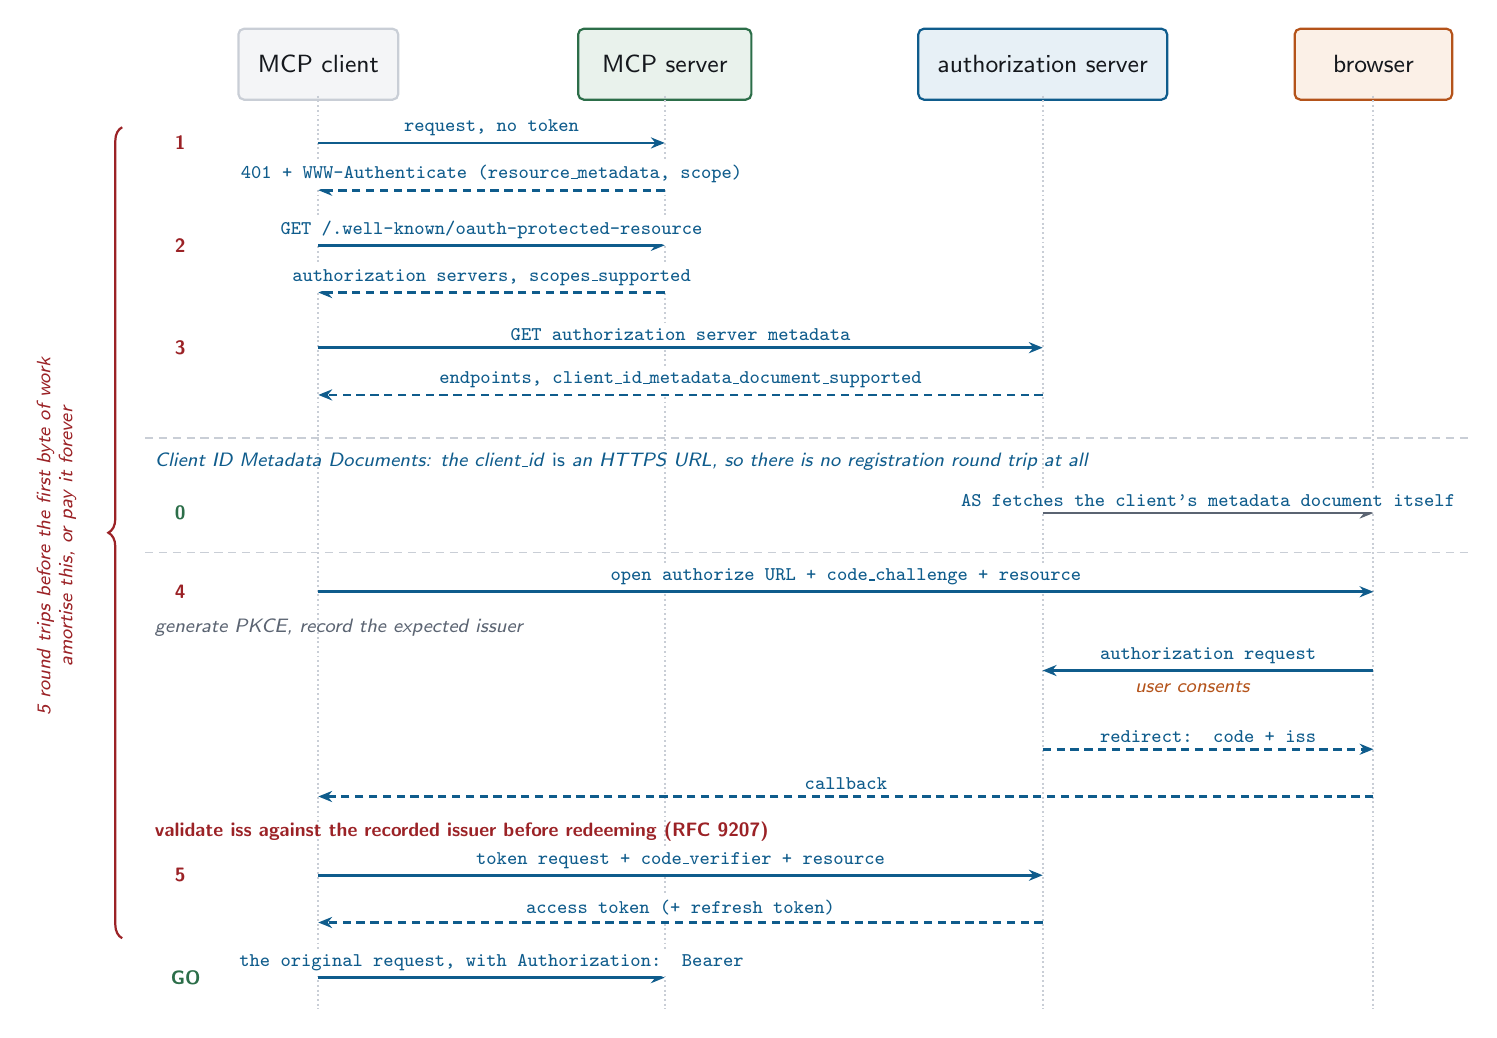
\begin{tikzpicture}[x=1cm, y=1cm]

  \def\C{0}      % client
  \def\M{4.4}    % MCP server (resource server)
  \def\A{9.2}    % authorization server
  \def\B{13.4}   % browser

  \node[box,  minimum width=20mm] (c) at (\C,0.6) {MCP client};
  \node[boxg, minimum width=22mm] (m) at (\M,0.6) {MCP server};
  \node[boxa, minimum width=26mm] (a) at (\A,0.6) {authorization server};
  \node[boxw, minimum width=20mm] (b) at (\B,0.6) {browser};

  \foreach \x in {\C,\M,\A,\B} { \draw[lifeline] (\x,0.2) -- (\x,-11.4); }

  \newcommand{\step}[5]{% from, to, y, style, label
    \draw[#4] (#1,#3) -- node[tag, above] {#5} (#2,#3);
  }

  % --- discovery ---------------------------------------------------------
  \node[lbl, anchor=west, text=danger] at (-1.9,-0.4) {\textbf{1}};
  \step{\C}{\M}{-0.4}{flow}{request, no token}
  \step{\M}{\C}{-1.0}{flowback}{401 + WWW-Authenticate (resource\_metadata, scope)}

  \node[lbl, anchor=west, text=danger] at (-1.9,-1.7) {\textbf{2}};
  \step{\C}{\M}{-1.7}{flow}{GET /.well-known/oauth-protected-resource}
  \step{\M}{\C}{-2.3}{flowback}{authorization servers, scopes\_supported}

  \node[lbl, anchor=west, text=danger] at (-1.9,-3.0) {\textbf{3}};
  \step{\C}{\A}{-3.0}{flow}{GET authorization server metadata}
  \step{\A}{\C}{-3.6}{flowback}{endpoints, client\_id\_metadata\_document\_supported}

  % --- registration ------------------------------------------------------
  \draw[draw=rule, line width=0.6pt, densely dashed] (-2.2,-4.15) -- (14.6,-4.15);
  \node[note, anchor=west, text=accent] at (-2.2,-4.45)
    {Client ID Metadata Documents: the client\_id \emph{is} an HTTPS URL, so
     there is no registration round trip at all};
  \node[lbl, anchor=west, text=good] at (-1.9,-5.1) {\textbf{0}};
  \step{\A}{\B}{-5.1}{flowmuted}{AS fetches the client's metadata document itself}

  % --- authorization -----------------------------------------------------
  \draw[draw=rule, line width=0.6pt, densely dashed] (-2.2,-5.6) -- (14.6,-5.6);
  \node[lbl, anchor=west, text=danger] at (-1.9,-6.1) {\textbf{4}};
  \node[note, anchor=west, align=left, text=muted] at (-2.2,-6.55)
    {generate PKCE, record the expected issuer};
  \step{\C}{\B}{-6.1}{flow}{open authorize URL + code\_challenge + resource}
  \step{\B}{\A}{-7.1}{flow}{authorization request}

  \node[note, anchor=south, text=warm] at (\A+1.9,-7.5) {user consents};
  \step{\A}{\B}{-8.1}{flowback}{redirect: code + \textbf{iss}}
  \step{\B}{\C}{-8.7}{flowback}{callback}

  \node[note, anchor=west, align=left, text=danger] at (-2.2,-9.15)
    {\textbf{validate iss against the recorded issuer before redeeming (RFC 9207)}};

  \node[lbl, anchor=west, text=danger] at (-1.9,-9.7) {\textbf{5}};
  \step{\C}{\A}{-9.7}{flow}{token request + code\_verifier + resource}
  \step{\A}{\C}{-10.3}{flowback}{access token (+ refresh token)}

  % --- the actual call ---------------------------------------------------
  \node[lbl, anchor=west, text=good, font=\sffamily\scriptsize\bfseries]
    at (-1.95,-11.0) {GO};
  \step{\C}{\M}{-11.0}{flow}{the original request, with Authorization: Bearer}

  % --- the cost tally ----------------------------------------------------
  \draw[decorate, decoration={brace, amplitude=5pt, raise=4pt}, danger, line width=0.8pt]
    (-2.35,-10.5) -- (-2.35,-0.2);
  \node[note, text=danger, rotate=90, anchor=south, align=center] at (-2.95,-5.4)
    {5 round trips before the first byte of work\\amortise this, or pay it forever};

\end{tikzpicture}
\end{document}
